\documentclass[10pt]{acmart}

\title{Extending Programming with Diagrammatic Programming Languages}
\author{Zac Nowicki}
\affiliation{
  \institution{Kagi Inc.}
  \city{Palo Alto}
  \state{CA}
  \country{USA}
}
\email{znowicki@kagi.com}

\author{Paul Tarvydas}
\affiliation{
  \institution{Retired}
  \city{Toronto}
  \state{Ontario}
  \country{Canada}
}
\email{paultarvydas@gmail.com}

\begin{document}

\begin{abstract}

  We assert that DPLs - Diagrammatic Programming Languages - can be used
  as an adjunct syntax for creating programs.

  We give an example of a simple DPL syntax and describe a method for
  creating executable code using diagrams drawn with off-the-shelf graphic
  editors.
  
  Certain forms of expression are more easily expressed in DPL form rather
  than TPL form. TPL-only expression of programs can lead to perceived
  complexity and increased program sizes. The use of DPLs makes it
  possible to address these sorts of issues using fresh notations.
\end{abstract}

\maketitle

\section{Introduction - Diagrams as Additional Syntax for Programming Languages}
The goal of programming is to create sequences of instructions -
programs - that cause electronic hardware to perform useful tasks.

To that end, programmers have been employing a single kind of syntax -
text.

Use of text for programs was based on the early limitations of
electronic hardware and on the convention that human thought needs to be
expressed as equations written on a two-dimensional medium - paper -
using printing presses.

Early electronic hardware was only capable of supporting grids of
non-overlapping bitmaps called "characters". Today, though, hardware can
support vector graphics and overlapping, resizable windows and widgets.

Early electronic hardware was made reprogrammable by the invention of
the Central Processing Unit - CPU. CPUs were originally designed to be
non-reentrant and single threaded. The high cost of early CPU-based
computers prevented use of multiple CPUs in projects, thus, causing the
insertion of extra software for simulating multiple CPUs on single
hardware devices. Today, though, CPUs - and memory - are inexpensive and
plentiful, a fact which should allow the use of alternate forms of
expressing programs.

The name "CPU" indicates the prevalent notion in early programming, that
hardware designs needed to be controlled by a central authority. This
belief is being strained as hardware becomes more distributed in the
form of internet, robotics, etc. The notion of centrality and
sequentiality was crystallized in early forms of TPL programming,
beginning at least with the FORTRAN programming language in 1954.

FORTRAN made the simplifying assumption that CPU subroutines could be
used to express mathematical equations ("formulae"). This assumption was
calcified and led to the invention of the callstack using shared memory.
Preemption was invented when the use of shared memory between
subroutines was found to conflict with the simulation of multiple CPUs.

These early kinds of expression continue to permeate most common
programming languages.

In essence, this paper shows that these habits of thought can be easily
re-cast using modern hardware and modern software.

This paper describes a technique for extending the syntax of programming
languages.

The new syntax consists of drawings containing simple, closed, graphical
figures and arrows.

We use the the name "DPL" - Diagrammatic Programming Languages - when
referring to this class of new programming syntax.

We assert that DPLs might be used \emph{along side} of existing TPLs (Textual
Programming Languages) and that DPLs are hybrids of diagram and textual
notations. TPLs are useful for expressing a specific kind of program -
computation - whereas other syntaxes make it more fruitful to express
other kinds of programs that don't lend themselves to being expresses in
equation form.

There are multiple possible DPL syntaxes. This paper suggests but a
single DPL syntax. It is assumed that a variety of syntaxes might be
invented, using the techniques described herein.

This paper touches on some of the key aspects of making compilable and
understandable drawings of programs, e.g. 0D, syntactic simplicity, DI
(Design Intent), etc.

We do not discuss fundamental DPL principles in this paper and refer the
reader to other related writings on these subjects.

This paper is laid out in 8 sections.

1. Introduction - Diagrams as Additional Syntax for Programming
Languages

2. Motivating Example

3. Leaf Component "Echo"

4. Compilation and Execution

5. Other Examples and Usage - lists brief descriptions and
code repositories for other POCs that employee this technique, along
with possible future directions.

6. Fundamental Principles - lays out the basic principles
for convenient development of programs

7. Relevant Principles and Issues - lists various
principles whose discussion is deferred.

8. Future - lists possible avenues for further research.

\section{Example}

  \begin{figure}[h]
    \centering
    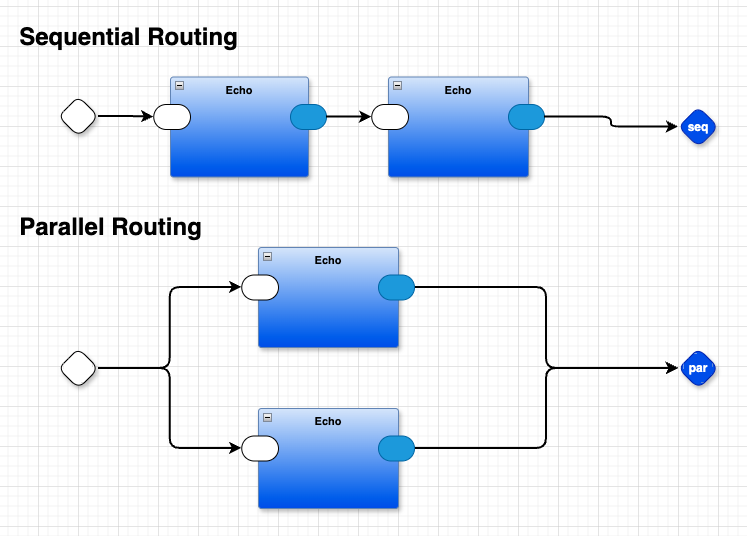
\includegraphics[width=0.8\linewidth]{./media/HelloWorld0D.png}
    \caption{Towards DPLs-1. Motivating Example}
    \label{fig:convert_to_json}
  \end{figure}

Fig. 1 shows but one sample of a practical DPL syntax. Variations and
improvements on this syntax can be imagined. This syntax is being used
to produce actual applications like term-rewriting (*t2t* -
text-to-text - rewriting) compilers, LLMs, DSLs for creating DSLs,
Visual Shell prototypes, games, etc.

This DPL syntax consists of only a few kinds of closed figures plus
arrows plus text belonging to the closed figures. Everything else is
considered to be a comment, and, is ignored. For example the bold text
"Sequential Routing" is ignored. Colors are ignored. Line shapes and
line widths are ignored, and so on.

This diagram was drawn using the off-the-shelf diagram editor
draw.io\cite{diagrams_net}. The editor saves the diagram in a modified form of XML, called \emph{graphML}\footnote{\url{https://en.wikipedia.org/wiki/GraphML}}.

The graphML file can be processed using off-the-shelf tools, like an XML parser or a PEG-based parser\footnote{\url{https://en.wikipedia.org/wiki/Parsing_expression_grammar}}\footnote{\url{http://ohmjs.org}}.

In our case, we used the Odin programming language\footnote{Odin} and the XML parsing library that is included in the Odin library\footnote{Odin XML parser}.

We choose not to reproduce the code for the actual diagram parser here, due to space limitations for this paper. The full source code for the functioning diagram parser is in an open-source repo\footnote{\url{https://github.com/guitarvydas/onward/tree/main/helloworld0d/0D/das2json}}.

The diagram parser produces internal data structures in the host programming language and/or JSON\footnote{JSON} files.

A \href{http://draw.io}{draw.io} file can contain several diagrams, each on a separate tab (window) in the editor.

The structure of the information needed by the DPL runtime is minimal, consisting of about four (4) fields for each diagram:

\begin{verbatim}
"file": "helloworld0d.drawio",
"name": "main",
"children": [
    {
    "name": "Echo",
    "id": 6
    },
... (2 more children referring to the same template "Echo", but assigned
Different ids) ...
],
"connections": [
    {
    "dir": 0,
    "source": {
    "name": "",
    "id": 0
    },
    "source_port": "",
    "target": {
    "name": "Echo",
    "id": 6
    },
"target_port": ""
},
... [7 more connections as per the diagram] ...
]
\end{verbatim}

The filename of the \href{http://draw.io}{draw.io} drawing

The tab-name of the top-most diagram.

A bag of Children components.

A bag of Connections between children (including connections to/from the parent containing diagram).

\section{Leaf Component "Echo"}
In our implementation, we used the Odin programming language for
creating the diagram parser, but, we used the Python programming
language to load and execute the parsed results.

Figure 1 refers to a Leaf component template called "Echo". The "Echo"
component is instantiated three (3) times. Leaf components are
implemented with code in some host language (Python, in our case). A
sample of such an implementation is shown below. Software components
appear as rectangles on the drawing. The implementation provides two (2)
entry points for each software component:

The code to instantiate a component from the "Echo" template. In Figure
1, the "Echo" code creates three (3) instances, each being unique, but,
derived from the same template.

The code to handle incoming messages for each instance derived from the
template. In this example, an "Echo" component does nothing more than
forwarding the received message. The \emph{handler} code is activated for
\emph{each} incoming message.

\begin{verbatim}
def Echo (reg, owner, name, template_data):
    name_with_id = gensym ("Echo")
    return make_leaf (name_with_id, owner, None, Echo_handler)

def Echo_handler (eh, msg):
    send_string (eh, "", msg.datum.srepr (), msg)
\end{verbatim}

\section{Compilation and Execution}
Compilation and execution of this DPL consists of the following steps:

\begin{enumerate}
\item Convert DPL program diagrams to JSON

  \begin{figure}[h]
    \centering
    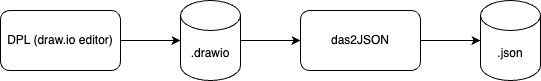
\includegraphics[width=0.8\linewidth]{./media/image2.png}
    \caption{Towards DPLs-1. Convert diagram to JSON}
    \label{fig:convert_to_json}
  \end{figure}

  Transpilation of the diagrams (XML) into JSON (or internal data structures, if efficiency is at a premium). The diagrams represent \emph{templates} for components.
  
  In our implementation, \texttt{das2json}\footnote{\url{https://github.com/guitarvydas/onward/tree/main/helloworld0d/0D/das2json}} is implemented\footnote{\url{https://github.com/guitarvydas/onward/tree/main/helloworld0d/0D/das2json}} in the Odin programming language. The process begins with a straightforward call to the XML parsing library. The XML data is then deconstructed into a convenient internal format (see \texttt{0d/ir/ir\_odin/ir.odin} in the code repository).

\begin{verbatim}
    xml, xml_err := xml.parse(file)
...
\end{verbatim}
  
\item Load component templates from JSON

  \begin{figure}[h]
    \centering
    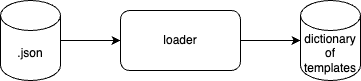
\includegraphics[width=0.6\linewidth]{./media/image3.png}
    \caption{Towards DPLs-2. Loader}
    \label{fig:load_templates}
  \end{figure}

  Ingestion of the JSON, or internal data structures into an internal database that we call a \emph{registry} (which can be implemented as a \emph{dictionary, map} or a \emph{database}).

\begin{verbatim}
    routings = json.loads(json_data)
...
\end{verbatim}

\item Instantiate system
  \begin{figure}[h]
    \centering
    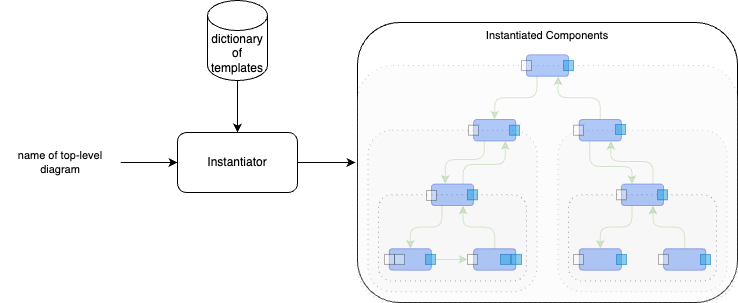
\includegraphics[width=0.8\linewidth]{./media/image4.png}
    \caption{Towards DPLs-3. Instantiate}
    \label{fig:instantiate_system}
  \end{figure}

  Instantiation\footnote{\url{https://github.com/guitarvydas/onward/blob/main/helloworld0d/0D/python/std/run.py}} of an application beginning with a top-level diagram
and proceeds downwards to instantiate all children components needed in
the top-level diagram and, recursively, instantiating the childrens'
children. Components are instantiated based on their DPL templates.
Containers are instantiated by instantiating all child components and
all routings between components. Note that more than one child component
can refer to the same DPL template. Components must be uniquely
instantiated - typically their (x,y) position is enough to differentiate
components, but, [[draw.io]{.underline}](http://draw.io) assigns unique
id's to each template component, which we ended up using instead of
relying on (x,y) graphical information. Assigning unique id's is a
convenience, not a requirement.


\begin{verbatim}
...
    main_container = get_component_instance(pregistry,
        main_container_name,
        owner=None)

...
\end{verbatim}

Software components are fully isolated from one another through the use
of FIFO queues.

\item Inject first message
  \begin{figure}[h]
    \centering
    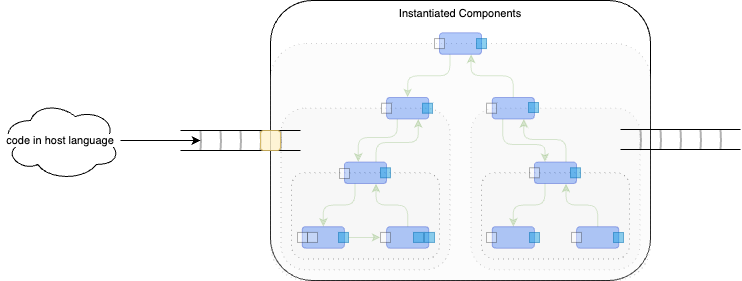
\includegraphics[width=0.8\linewidth]{./media/image5.png}
    \caption{Towards DPLs-4. Inject first message(s)}
    \label{fig:inject_first_message}
  \end{figure}

The first message is constructed using the host language. The message is
injected\footnote{\url{https://github.com/guitarvydas/onward/blob/main/helloworld0d/main.py}} into the input queue of the top-most component.

\begin{verbatim}
...
def start_function (root_project, root_0D, arg, main_container):
    arg = new_datum_string (arg)
    msg = make_message(\"\", arg)
    inject (main_container, msg)
...
\end{verbatim}
  
\item Run
  \begin{figure}[h]
    \centering
    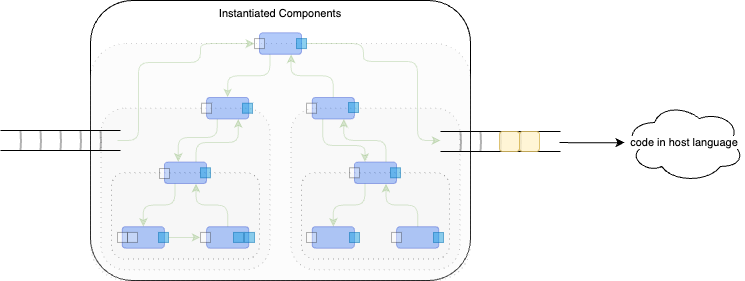
\includegraphics[width=0.8\linewidth]{./media/image7.png}
    \caption{Towards DPLs-5. Run}
    \label{fig:run}
  \end{figure}
The application is executed.

The application is interpreted by repeatedly delivering messages along
connections, recursively, until no messages remain in any input queues.

\emph{It is possible to invoke already-written library code written in some other host language using an activity indicator - see the code repo for more details.}

Containers must consume only one input message at a time while waiting
for all children to reach quiescence.

\begin{verbatim}
...
    if not load\_errors:
        injectfn (root_project, root_0D, arg, main_container)
...
\end{verbatim}
  
\item Display outputs
  \begin{figure}[h]
    \centering
    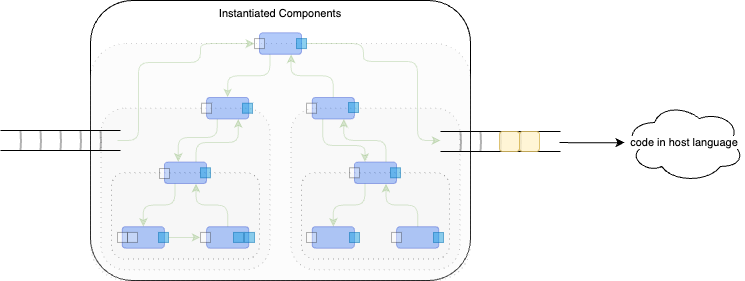
\includegraphics[width=0.8\linewidth]{./media/image7.png}
    \caption{Towards DPLs-6. Display Outputs}
    \label{fig:display}
  \end{figure}

The outputs in the output queue of the top-level component are displayed
using the host language.

\begin{verbatim}
...
    dump_outputs (main\_container)
...
\end{verbatim}
  
\end{enumerate}

The Python version of the runtime system consists of roughly 9 files of
code consisting of about 2,500 lines of code (including blank lines and
comments) and is supported by a standard library consisting of another 5
files of code containing about 430 lines of code.

At the basic level, runtime component instances are asynchronous, but,
use named and anonymous functions and closures, instead of operating
system processes. As such, programs written this way "feel" like
\emph{programs} instead of as \emph{processes} in terms of efficiency.

\section{Other Examples and Usage}
We have built working examples of various other technologies, using the
DPL described in this paper, including,

\begin{itemize}
\item VSH a Visual SHell that works like /bin/sh pipelines employing more input and output ports,
\item arith0d OhmJS' arithmetic grammar that concurrently emits four (4) target languages (Javascript, Python, Common Lisp, WASM),
\item LLM0D a single component diagram that uses the Go programming language as a host language to connect to openai's LLM for experimenting with LLMs,
\item transpiler a workbench for creating new textual syntaxes, uses OhmJS more than once in a pipeline
\item kinopio2md experiment for converting Kinopio "mindmaps" into markdown based on connections between ideas expressed in Kinopio
\item Scheme to Javascript, Scheme to Python - conversion of Nils Holm's Scheme code used in "Prolog Control Flow in 6 Slides" to produce a Prolog-like inferencing engine for Javascript, currently working on conversion to Python
\item delay0d
\item Dc0d game engine based on Chris Marten's "dungeon crawler" example\cite{ceptre_paper}; including gen0D generates components (in Odin) from the diagram (instead of interpreting the diagram, gen0D creates leaf components that are used in conjunction with the diagram)
\item 0D odin a DPL engine written in the Odin programming language (Odin is statically typed, and, does not provide garbage collection, similar to languages like C)
\item Crystal 0D a DPL engine written in the Crystal programming language, which is currently being used in a production system
\item 0D cookbook ongoing effort to document all standard DPL components as \href{http://draw.io}{draw.io} diagrams
\end{itemize}

\section{Fundamental Principles}
Software components are fully isolated from one another through the use
of FIFO queues. Using the LIFO callstack for inter-component
communication leads to hidden dependencies which leads to avoidance of
DPLs.

There is exactly one input queue and one output queue per component. We
do not use, for semantic reasons, one queue per port. In general, single
queues allow programs to track relative time-ordering of messages - an
important feature when programming devices that perform sequencing
instead of computation. In addition, multiple queues can lead to
deadlock issues. These issues still exist in the large, but are
mitigated through the use of single input and output queues and tend not
to occur in hidden, unexpected ways.

\section{Relevant Principles and Issues}
We do not discuss the following principles in detail in this paper, due
to reasons of space.

\begin{itemize}
\item Structured Message Passing
\item Rule of 7
\item Parental Authority
\item No built-in paradigm. Async and ordered-in-time by default.
\item SEND in addition to CALL
\item Locality of Reference
\item Scoping of names
\item Every diagram is stable, every diagram can be understood on its own.
Children cannot change the behaviour of their parents.
\item All components are asynchronous by default.
\item CPUs are meant to be single-threaded
\item There is no single happy path in many applications
\item Subroutines are not functions
\item Hidden dependencies
\item Build-and-forget
\item LEGO® block-like composition of software components (needs full
isolation).
\item Modern tooling for developers, breaking free of the function-based
paradigm.
\item Building new paradigms using existing tools.
\item \emph{t2t} text-to-text transpilation pipelines.
\end{itemize}

\section{Future}
\begin{itemize}
\item Compilation, instead of interpretation, to other languages.

\item Parsing XML using the \emph{Transpiler} component instead of calling XML parsing libraries.

\item Testing, unit testing, coverage testing.

\item Depending on the graphical editor used, Prolog (among other languages)
can be used to inference semantic information.
\end{itemize}

\section{References}

\begin{thebibliography}{9}
\bibitem{diagrams_net}
Diagrams.net.
\url{https://app.diagrams.net}
\bibitem{ceptre_paper}
Martens, Chris. Ceptre: A Language for Modeling Generative Interactive Systems. \url{https://www.cs.cmu.edu/~cmartens/ceptre.pdf} (Accessed: January 19, 2024).
\end{thebibliography}

\begin{enumerate}
\item \href{https://app.diagrams.net/}{https://app.diagrams.net/}
\item \href{https://en.wikipedia.org/wiki/GraphML}{https://en.wikipedia.org/wiki/GraphML}
\item \href{https://en.wikipedia.org/wiki/Parsing_expression_grammar}{https://en.wikipedia.org/wiki/Parsing\_expression\_grammar}
\item \href{http://ohmjs.org}{ohmjs.org}
\end{enumerate}

\end{document}
